\documentclass{tufte-handout}

\title{Descriptive Statistics Review}

%\author[The Tufte-LaTeX Developers]{The Tufte-\LaTeX\ Developers}

\date{} % without \date command, current date is supplied


\usepackage{graphicx} % allow embedded images
  \setkeys{Gin}{width=\linewidth,totalheight=\textheight,keepaspectratio}
  \graphicspath{{graphics/}} % set of paths to search for images
\usepackage{amsmath}  % extended mathematics
\usepackage{booktabs} % book-quality tables
\usepackage{units}    % non-stacked fractions and better unit spacing
\usepackage{multicol} % multiple column layout facilities
\usepackage{lipsum}   % filler text
\usepackage{fancyvrb} % extended verbatim environments
  \fvset{fontsize=\normalsize}% default font size for fancy-verbatim environments

\usepackage{pgfplots}
\pgfplotsset{compat=1.12}

% Standardize command font styles and environments
\newcommand{\doccmd}[1]{\texttt{\textbackslash#1}}% command name -- adds backslash automatically
\newcommand{\docopt}[1]{\ensuremath{\langle}\textrm{\textit{#1}}\ensuremath{\rangle}}% optional command argument
\newcommand{\docarg}[1]{\textrm{\textit{#1}}}% (required) command argument
\newcommand{\docenv}[1]{\textsf{#1}}% environment name
\newcommand{\docpkg}[1]{\texttt{#1}}% package name
\newcommand{\doccls}[1]{\texttt{#1}}% document class name
\newcommand{\docclsopt}[1]{\texttt{#1}}% document class option name
\newenvironment{docspec}{\begin{quote}\noindent}{\end{quote}}% command specification environment


\begin{document}

\maketitle% this prints the handout title, author, and date


%\printclassoptions

\section{Measurement Scales and their Properties}

\begin{table}
  \centering
  \fontfamily{ppl}\selectfont
  \begin{tabular}{lllll}
    \toprule
    Scales & Properties & Examples \\
    \midrule
    Categorical/Nominal & Identity & gender, political affiliation\\
    Ordinal & +Magnitude & rank ordering, e.g. placement in a race\\
    Interval & +Equal Unit Size & Fahrenheit or Celsius\\
    Ratio & +Absolute Zero & time, weight, height, Kelvin\\
    \bottomrule
  \end{tabular}
  \label{tab:normaltab}
  %\zsavepos{pos:normaltab}
\end{table}


\section{Frequency Distributions}

\begin{table}
  \centering
  \fontfamily{ppl}\selectfont
  \begin{tabular}{lllll}
    \toprule
    Frequency & $f$ & how many times a score occurs\\
    Proportion & $f/n$ & where $n$ is the sample size\\
    Cumulative Frequency & $cf$ & number of scores $\leq$ a given value\\
    Cumulative Proportion & $cp=\frac{cf}{n}$ \\
    \bottomrule
  \end{tabular}
  \label{tab:normaltab}
  %\zsavepos{pos:normaltab}
\end{table}

\begin{margintable}[4.0in]
  \centering
  \fontfamily{ppl}\selectfont
  \begin{tabular}{rrr}
    \toprule
    $x$ & $f$ & $cf$\\
     0  &   4 &    4\\
     1  &   8 &   12\\
     2 &   12&    24\\
     3 &   10&    34\\
     4 &    5 &   39\\
     5 &    6 &   45\\
     6 &    2 &   47\\
     7 &    2 &   49\\
     8 &    1 &   50\\
     9 &    0 &   50\\
    \bottomrule
  \end{tabular}
  \label{tab:normaltab}
\end{margintable}

\begin{figure}%
  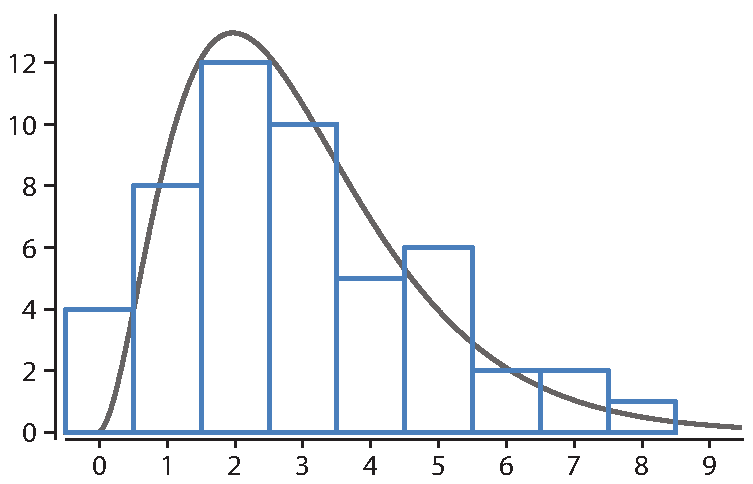
\includegraphics[width=\linewidth]{images/handout1_hist}%
  \label{fig:fullfig}%
  \caption{A histogram for a unimodal distribution with positive skew. Bars denote data from 50 observations, curve denotes an underlying smooth distribution.}
\end{figure}

\section{Describing the Shape of a Distribution}
\begin{fullwidth}
\begin{description}
\item[1.] A distribution is \emph{symmetric} if there is an axis about which the tails are the same\\
\item[2.] \emph{Skewness} quantifies asymmetry: positive skew (long right tail) vs negative skew (long left tail)\\
\item[3.] \emph{Modality}: how many peaks are there (e,g, unimodal, bimodal, multimodal)\\
\end{description}
\end{fullwidth}

\section{Descriptive Statistics Summary}

\begin{fullwidth}
Measures of Central Tendency:	
\begin{description}
\item[1.] Mean: Average, sensitive to outliers
\item[2.] Median: 50th percentile, insensitive to outliers, but not as useful in statistical inference
\item[3.] Mode: Most frequent value, peak(s) of a smooth distribution
\end{description}
\end{fullwidth}

\begin{align*}
&\text{Sample Mean} & \bar{X}&=\frac{\sum X}{n}\\
&\text{Sum of Squares} & SS&=\sum (X-\bar{X})^2\\
&\text{Sample Variance} & s^2&=\frac{\sum (X-\bar{X})^2}{n-1} = \frac{SS}{n-1}\\
&\text{Sample Standard Deviation} & s&=\sqrt{\frac{\sum (X-\bar{X})^2}{n-1}}=\sqrt{s^2}\\
&\text{Population Mean} & \mu&=\frac{\sum X}{N}\\
&\text{Population Variance} & \sigma^2&=\frac{\sum (X-\mu)^2}{N}\\
\end{align*}

\begin{fullwidth}
Notes: $s^2$ is calculated using $n-1$. Using $n$ yields a biased estimator. $N$ is the population size.
\end{fullwidth}

\begin{align*} 
&\text{Percentile Rank} & &\frac{cf-0.5f}{n} \cdot 100 \% \\
&\text{Range} & &max(X)-min(X)\\
&\text{Inter-quartile Range} & &75^{th}-25^{th} \text{percentile (or Q3-Q1)}\\
\end{align*}

\begin{figure}%
  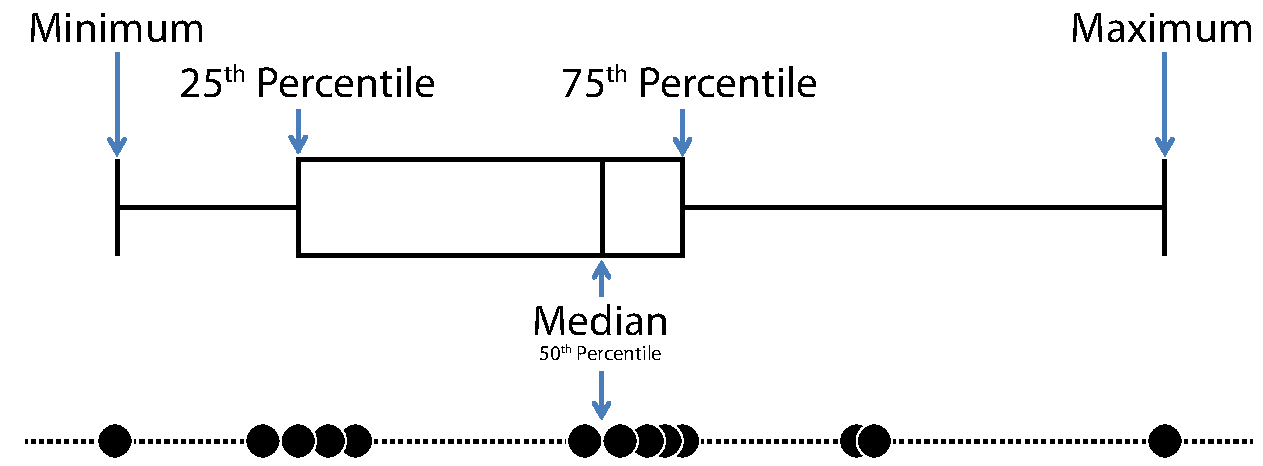
\includegraphics[width=\linewidth]{images/handout1_boxplot}%
  \label{fig:fullfig}%
  \setfloatalignment{b}
  \caption{Box Plot. Whiskers often use different standards, such as 1.5xIQR, and attempt to remove outliers.}
\end{figure}

\end{document}
